\documentclass[a4paper]{article}
\usepackage[a4paper,pdftex]{geometry}
\usepackage[english]{babel}
\usepackage{amsmath,amsfonts}
\usepackage[pdftex]{graphicx}
\usepackage{epstopdf}
\usepackage{fancyhdr}
\usepackage{lastpage}

% Page margins
%\setlength{\oddsidemargin}{5mm}
%\setlength{\evensidemargin}{5mm}

% Page style
\pagestyle{plain}

% Page numbering
\lhead{Sensor Fusion on a mini Unmanned Vehicles - Camiel R. Verschoor}
\cfoot{}
\rfoot{\thepage}

% TITLE FORMAT
\newcommand{\HRule}[1]{\rule{\linewidth}{#1}}

\makeatletter
\def\printtitle{
    {\centering \@title\par}}
\makeatother                  

\makeatletter
\def\printauthor{
    {\centering \large \@author}}
\makeatother

% TITLE
\title{
\HRule{0.5pt} \\
\LARGE \textbf{\textsc{Sensor Fusion on a mini Unmanned Vehicle}}\\[0.5cm]
\normalsize \textsc{Integrating vision-based algorithms on an AscTec Pelican to autonomously follow linear shaped structures in a landscape.}
\HRule{2pt}\\ [0.5cm]
Camiel R. Verschoor\\
10017321\\
\vspace{1cm}
Bachelor thesis\\
Credits: 18 EC\\
\vspace{0.5cm}
Bachelor Opleiding Kunstmatige Intelligentie\\
\vspace{0.25cm}
University of Amsterdam\\
Faculty of Science\\
Science Park 904\\
1098 XH Amsterdam\\
}

% AUTHOR
\author{\normalsize
\emph{Supervisors}\\
Dr. A. Visser\\
\vspace{0.25cm}
Informatics Institute\\
Faculty of Science\\
University of Amsterdam\\
Science Park 904\\
1098 XH  Amsterdam\\
\vspace{0.5cm}
Drs. G. Poppinga\\
\vspace{0.25cm}
Defense Systems (ASMO)\\
National Aerospace Lab\\
Anthony Fokkerweg 2\\
1059 CM Amsterdam\\
\vspace{1cm}
July 24th, 2012\\
}

% BEGIN DOCUMENT
\begin{document}

% TITLE PAGE
\thispagestyle{empty}
\printtitle
\vfill          
\printauthor
\newpage

% ABSTRACT
\section*{Abstract}
To be written.
\section*{Acknowledgements}
To be written.
\newpage

% TABLE OF CONTENTS
\tableofcontents
\newpage

\section{Introduction}
In robotics one of the main goals is to develop mobile robots that can operate autonomously in the real world environment. These autonomous robots have various purposes and are used for a wide range of applications such as inspection, exploration or rescue. In rescue the robot is expected to operate in dangerous environments without putting human lives in danger in example, during disasters or life rescue operations. Even though reasonable developments have been made in the robotics field, robots cannot operate autonomously in the real world yet.

One of the main requirements of an autonomous robot is the ability to navigate in the environment. The traditional approach to navigate through the outdoor environment is via pre-planned paths based on a Global Positioning System (GPS). The main shortcoming of GPS is that it cannot be used in every environment as it needs to receive a data signal from four different satellites. Inside buildings and in several outdoor areas GPS is not available. Especially in urban areas GPS is found to be unreliable. In order to navigate through these environments other sensors and navigation techniques should be applied. Since there are several linear structures in the environment like rivers, roads and power lines, line-following is a possible approach to navigate through an environment. Line-following is a classic technique in robotics as it has been used for ground robots successfully several times. For other robots and sensor configurations, open problems remain. One of them is navigation for micro aerial vehicles (MAVs), which have a limited sensor composition due to their limited payload.

\begin{figure}[!h]
	\centering
	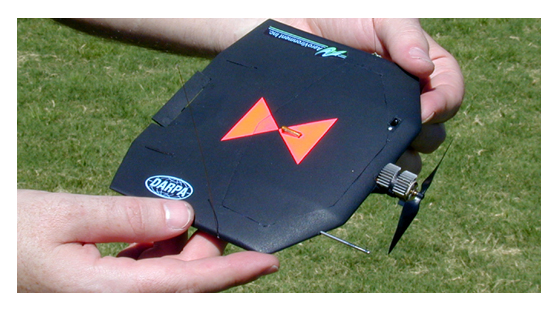
\includegraphics[width=0.5\textwidth]{images/blackwidow.eps}
	\caption{The Black Widow was the first operating micro aerial vehicle system developed by AeroVironment for Defense Advanced Research Projects Agency (DARPA). The Black Widow can fly for up to 20 minutes and carries a very small color video camera.}
	\label{blackwidow}
\end{figure}

A micro aerial vehicle (MAV) is a subclass of the Unmanned Aerial Vehicles. Due to their small size, the MAV can operate in numerous robotic applications. For instance, search \&  rescue, inspection and exploration. AeroVironment Black Widow (figure \ref{blackwidow}) is the first MAV operating in the field. Another type of MAV is the quadrotor, which is controlled by four rotors. Quadrotors provide  
manoeuvrability and stability, which is quintessential for indoor and urban flights. As a result of recent developments, small quadrotors with on-board stabilization can be purchased conveniently. Due to this, the research regarding this platform is moving towards intelligent applications, which demand information of the surrounding environment. Nevertheless, the fast movements and the limited amount of sensor combination it is still a challenge to use navigation method for these platforms.

\subsection{Line following}
Line following experiment.
\subsection{Research questions and objectives}
The main research question is to find a robust vision-based approach to autonomously navigate over linear shaped structures. This main research question is divided up in the following sub-questions:
\begin{itemize}
\item What vision-based algorithms are suitable for robust  
\item Question
\end{itemize}
\subsection{Platform}
Ascending Technologies Pelican.
\subsection{Framework}
\subsection{Outline}
Chapter X gives an overview about current used vision-based methods...
To be written.



\end{document}
